% $Id$
% !Mode:: "TeX:DE"    % Setting document mode and submode for WinEdt
% ..............................................................................
%                  E L L I P T I S C H E  K U R V E N
% ~~~~~~~~~~~~~~~~~~~~~~~~~~~~~~~~~~~~~~~~~~~~~~~~~~~~~~~~~~~~~~~~~~~~~~~~~~~~~~

\begin{refsegment}

\newpage
\hypertarget{Chapter_EllipticCurves}{}
\chapter{Elliptische Kurven}
\label{Chapter_EllipticCurves}
\index{elliptische Kurve}
(\hyperlink{author_Bartol-Filipovic}{Bartol Filipovic} /
 \hyperlink{author_Matthias-Bueger}{Matthias Büger} /
 \hyperlink{author_Bernhard-Esslinger}{Bernhard Esslinger} /
 \hyperlink{author_Roger-Oyono}{Roger Oyono},
 April 2000,
 Updates: Dez. 2001, Juni 2002, März 2003, Nov. 2009, Aug. 2013, Aug. 2016)

% -----------------------------------------------------------------------------
\section{Elliptische Kurven -- Ein effizienter Ersatz für RSA?}
\index{Performance}
\label{ECAlternative}

Bei Datenübertragungen kommt es auf Sicherheit und Effizienz an.  Viele
Anwendungen verwenden den RSA-Algorithmus als asymmetrisches Signatur- und
Verschlüsselungsverfahren.

Solange die verwendeten Schlüssel hinreichend lang sind, bestehen keinerlei
Bedenken gegen die {\em Sicherheit} des RSA-Verfahrens. Allerdings hat die
Entwicklung der Rechnerleistungen in der vergangenen Jahren dazu geführt,
dass die benötigten Schlüssellängen mehrfach angehoben werden mussten
(vergleiche Kapitel \ref{SecurityRSA}).
Da die meisten Chips auf Smartcards\index{Smartcard} nicht in der Lage sind,
längere Schlüssel als z.B. 2000 Bit zu verarbeiten, besteht Bedarf für
Alternativen zum RSA. Eine solche Alternative sind Elliptische Kurven. Diese
werden inzwischen auch auf Smartcards eingesetzt.

Die {\em Effizienz} eines kryptographischen Algorithmus hängt wesentlich
von der benötigten \linebreak[4]Schlüssellänge und vom Rechenaufwand ab,
um ein vorgeschriebenes Sicherheitsniveau zu erreichen.
Der entscheidende Vorteil Elliptischer Kurven im Vergleich zum
RSA-Algorithmus liegt in der Tatsache, dass die sicheren Schlüssellängen
erheblich kürzer sind.

Setzt man den Trend, dass sich die Leistung der verfügbaren Rechner im
Schnitt alle 18 Monate verdoppelt (vgl.\ dazu das Gesetz von
Moore\index{Gesetz von Moore}\index{Moore, Gordon E.}\footnote{%
  Das Mooresche Gesetz formuliert die empirische Beobachtung und die darauf
  aufbauende Prognose, dass sich die Anzahl der Komponenten bzw. Transistoren
  in einer integrierten Schaltung alle zwei Jahre verdoppelt. Es bezog sich
  ursprünglich nur auf die Transistorendichte in einer integrierten Schaltung,
  aber bspw. nicht auf den Zuwachs bei der Speicherdichte.
  Diese Erkenntnis zur Transistorendichte wurde 1965 (mit einer Korrektur 1975)
  von Gordon Moore, einem Mitbegründer von Intel, geäußert.
  In den letzten Jahren war der Zuwachs an Computerleistung sogar höher als
  die prognostizierte Verdopplung alle 2 Jahre. Grenzen setzt in Zukunft die
  Transistorengröße von wenigen Atomen, die bis zum Jahr 2020 erreicht werden könnte.
}% Siehe: https://de.wikipedia.org/wiki/Mooresches_Gesetz
), in die Zukunft fort, so kann man von einer Entwicklung der
sicheren Schlüssellängen wie in Abbildung~\ref{RSAKeylength} ausgehen,
die anhand der Tabelle 1 (auf Seite 32 in \cite{LeVe2001}) erstellt
wurde.\footnote{%
  Weitere Informationen zum Schlüssellängen-Vergleich von Arjen Lenstra und
  Eric Verheul, aber auch zu neueren Untersuchungen bis 2015 finden sich
  in der interaktiven Darstellung auf \url{https://www.keylength.com}.
  % \url{https://infoscience.epfl.ch/record/164539/files/NPDF-32.pdf}\\
  % Key Lengths, Arjen K. Lenstra, The Handbook of Information Security, 06/2004.
}

% -> Figure 1
\begin{figure}[ht]
\begin{center}
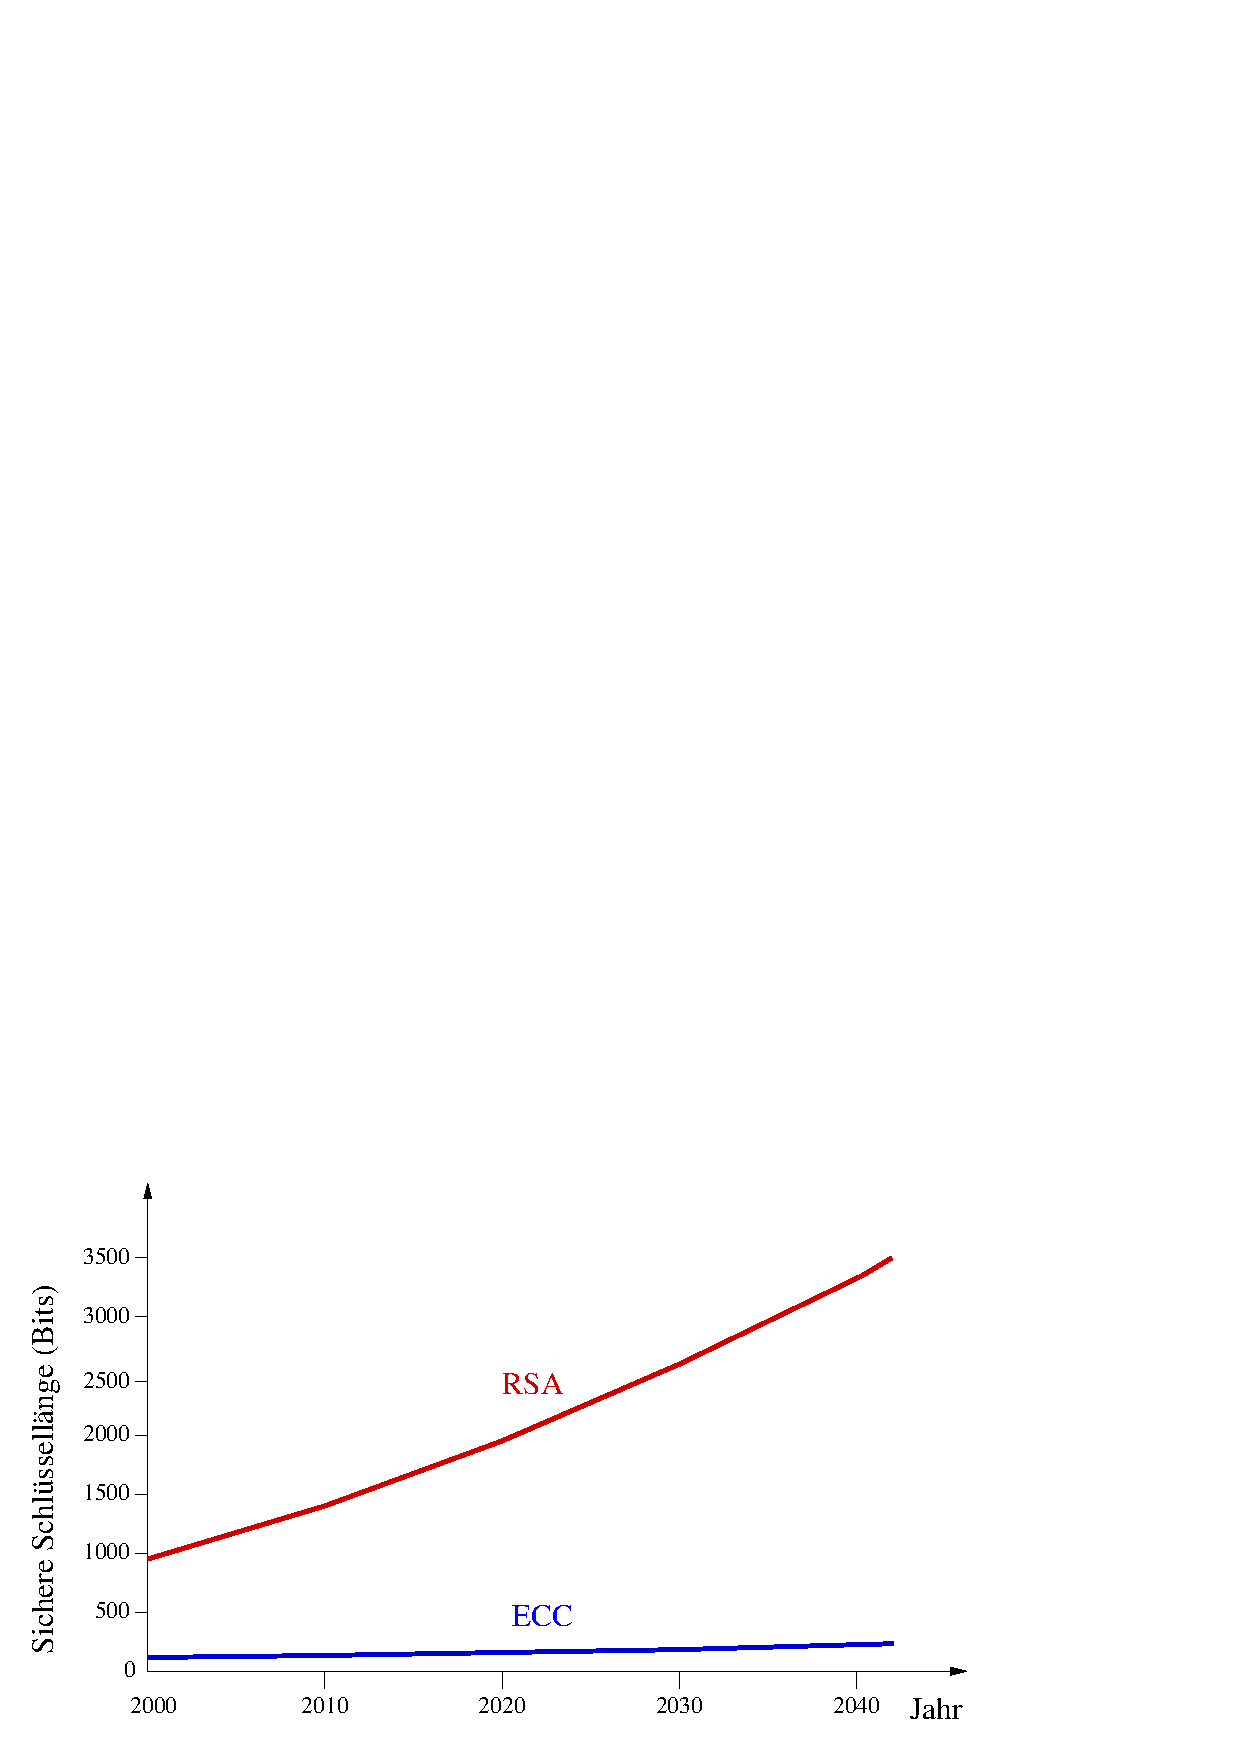
\includegraphics[scale=0.7]{figures/RSAKeyLength-2}
\caption{Prognose für die Entwicklung der als sicher betrachteten
  Schlüssellängen bei RSA und bei Elliptische Kurven}
\label{RSAKeylength}
\end{center}
\vskip -30 pt
\end{figure}

\newpage

Bei der digitalen Signatur muss man differenzieren: für die {\em
  Erstellung} einer digitalen Signatur benötigen auf Elliptischen
Kurven basierende Verfahren im Vergleich zu RSA nur gut ein Zehntel des
Rechenaufwands (66 zu 515 Ganzzahlmultiplikationen). Siehe hierzu
Abbildung~\ref{ThousandBitMultiplications} (Quelle: J.  Merkle,
Elliptic Curve Cryptography Workshop, 2001). Betrachtet man die für eine
{\em Verifikation} durchzuführenden Rechenschritte, dreht sich dieses Bild
jedoch zu Gunsten von RSA um (112 zu 17 Ganzzahlmultiplikationen). Der
Grund liegt darin, dass es bei Verwendung des RSA möglich ist, einen sehr
kurzen Exponent für den öffentlichen Schlüssel zu wählen, solange der
private Exponent nur hinreichend lang ist.

% -> Figure 2
\begin{figure}[ht]
\vskip -40 pt
\begin{center}
\vspace{1.5cm}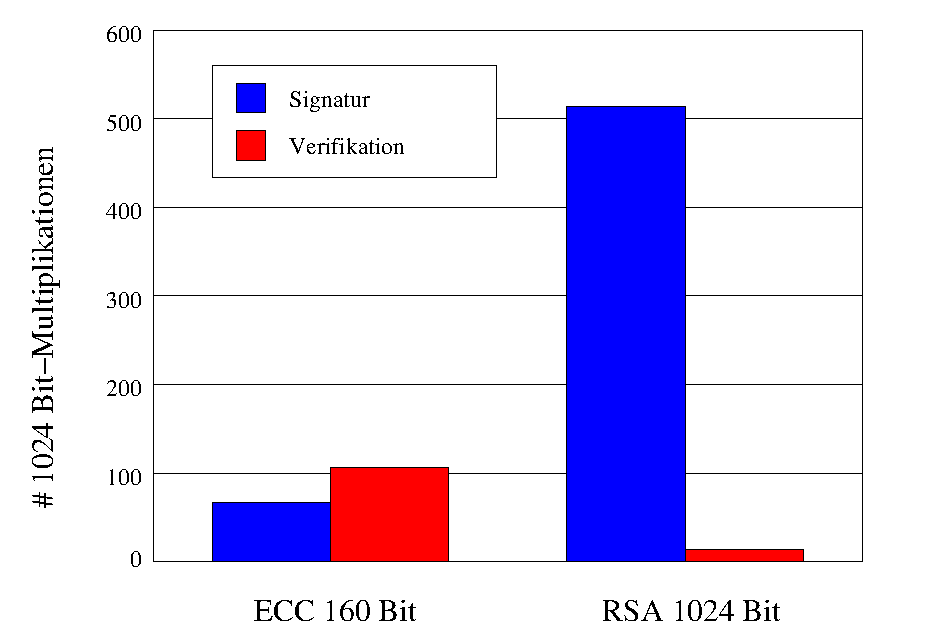
\includegraphics[scale=0.7]{figures/ECCRSA}
\caption{Gegenüberstellung des Aufwands der Operationen Signieren und
         Verifizieren bei RSA und bei Elliptischen Kurven}
\label{ThousandBitMultiplications}
\end{center}
\vskip -10 pt
\end{figure}

Da bei Smartcards, die auf RSA basieren, stets der lange (private)
Schlüssel auf der Karte gespeichert werden muss und die Erstellung
der digitalen Signatur, nicht aber die Verifikation, auf der Karte
stattfindet, treten hier deutlich die Vorteile Elliptischer Kurven zutage.
\par
\smallskip
Das größte Problem bei der Implementierung von Verfahren, die auf Elliptischen Kurven beruhen, ist bislang die
mangelnde {\em Standardisierung\index{Standardisierung}}. Es gibt nur eine RSA-Implementierung, aber viele Arten, Elliptische Kurven einzusetzen.
So können verschiedene Zahlkörper zugrunde gelegt, eine Vielzahl von (Elliptischen) Kurven --- durch
Parameter beschrieben\footnote{%
Siehe Kapitel \ref{ECC-Crypto}
} --- eingesetzt und unterschiedliche Darstellungen der Kurvenpunkte verwendet werden.
Jede Wahl hat ihre Vorzüge, so dass für jede Anwendung eine andere Implementierung optimal sein kann. Dies
hat jedoch zur Konsequenz, dass Systeme, die auf Elliptischen Kurven beruhen, oftmals nicht interoperabel
sind. Um mit einer beliebigen auf Elliptischen Kurven basierenden Anwendung kommunizieren zu können, müsste man
eine Vielzahl von Implementierungen vorhalten, was den Effizienzvorteil gegenüber der Verwendung von RSA
zunichte macht.

Deshalb bemühen sich internationale Organisationen um Standardisierung:
IEEE (P1363), ASC (ANSI X9.62, X9.63), ISO/IEC sowie
RSA Laboratories\index{RSA Laboratories} und Certicom\index{Certicom}.
Im Gegensatz zur IEEE, die bisher nur eine Beschreibung der verschiedenen
Implementierungen vorgenommen hat, hat die ASC konkret 10 Kurven ausgewählt
und empfiehlt deren Verwendung. Der Vorteil des ASC-Ansatzes ist,
dass ein einziges Byte ausreicht, um die verwendete Kurve zu spezifizieren.
Zur Zeit ist jedoch nicht absehbar, ob es der ASC gelingen wird, einen
de-facto-Standard durchzusetzen.

Obwohl aktuell kein Handlungsbedarf besteht\footnote{%
  Aktuelle Informationen zur Sicherheit des RSA-Verfahrens finden Sie in
  den Kapiteln \ref{SecurityRSA} und \ref{Chapter_Dlog-FactoringDead}.
},
laufende RSA-Anwendungen umzustellen, sollte man ernsthaft den Einsatz
von Elliptischen Kurven erwägen\footnote{%
  Siehe bspw. die Technische Richtlinie des BSI \glqq Kryptographische Verfahren:
  Empfehlungen und Schlüssellängen\grqq~vom 15. Februar 2016.
}.
Neuere Diskussionen zur Sicherheit von ECC finden Sie in Kapitel
\ref{Chapter_Dlog-FactoringDead}.


% -----------------------------------------------------------------------------
\section{Elliptische Kurven -- Historisches}

Auf dem Gebiet der Elliptischen Kurven wird seit über 100 Jahren geforscht. Im Laufe der Zeit hat man
viele weitläufige und mathematisch tiefgründige Resultate im Zusammenhang mit Elliptischen Kurven gefunden
und veröffentlicht. Ein Mathematiker würde sagen, dass die Elliptischen Kurven
(bzw.\ die dahinterstehende Mathematik) gut verstanden sind. Ursprünglich war diese Forschung reine
Mathematik, das heißt Elliptische Kurven wurden zum Beispiel in den mathematischen Teilgebieten
Zahlentheorie und algebraische Geometrie untersucht, die allgemein sehr abstrakt sind. Auch in der
nahen Vergangenheit spielten Elliptische Kurven eine bedeutende Rolle in der reinen Mathematik. In den
Jahren 1993 und 1994\footnote%
{
  1994 wurden die Beweislücken durch Wiles und Richard Taylor geschlossen.
}
veröffentlichte Andrew Wiles\index{Wiles, Andrew} mathematische Arbeiten, die weit über das Fachpublikum
hinaus auf große Begeisterung gestoßen sind. In diesen Arbeiten bewies er die Richtigkeit einer --- in
den sechziger Jahren des 20. Jahrhunderts von zwei Japanern aufgestellten --- Vermutung. Dabei geht es
kurz und grob gesagt um den Zusammenhang zwischen Elliptischen Kurven und sogenannten Modulformen.
Das für die meisten eigentlich Interessante daran ist, dass Wiles mit seinen Arbeiten auch den berühmten
zweiten Satz von Fermat\index{Fermat!letzter Satz} bewiesen hat. Dieser Satz hatte sich seit Jahrhunderten
(Fermat\index{Fermat, Pierre} lebte von 1601 bis 1665) einem umfassenden Beweis durch die Mathematik
entzogen. Dementsprechend
groß war die Resonanz auf den Beweis durch Wiles. In der Formulierung von Fermat lautet der nach ihm
benannte Satz so (Fermat hat folgende Worte an den Rand des 1621 von Bachet de Meziriac
herausgegebenen Werks von Diophant geschrieben):

\begin{quote} {\em
Cubum autem in duos cubos, aut quadratoquadratum in duos quadratoquadratos, et
generaliter nullam in infinitum ultra quadratum potestatem in duos ejusdem nominis
fas est dividere: cujus rei demonstrationem mirabilem sane detexi. Hanc marginis
exiguitas non caperet.
} \end{quote}

Frei übersetzt und mit der Schreibweise der heutigen Mathematik bedeutet dies:\\
Es gibt keine positiven ganzen Zahlen $x, y$ und $z$ größer als Null, so dass
$x^n + y^n = z^n$ für $n>2$ gilt.
Ich habe einen bemerkenswerten Beweis für diese Tatsache gefunden, aber es ist
nicht genug Platz am Rand [des Buches], um ihn niederzuschreiben.

Dies ist schon bemerkenswert: Eine relativ einfach zu verstehende Aussage
(gemeint ist Fermats zweiter Satz) konnte erst nach so langer Zeit bewiesen werden, obwohl
Fermat selber angab, schon einen Beweis gefunden zu haben.
Im übrigen ist der Beweis von Wiles sehr umfangreich (alle im Zusammenhang mit dem Beweis
stehenden Veröffentlichungen von Wiles ergeben schon ein eigenes Buch). Man sollte sich daher
im klaren sein, dass die Elliptischen Kurven im allgemeinen sehr tiefgreifende Mathematik berühren.

Soweit zur Rolle der Elliptischen Kurven in der reinen Mathematik.
Im Jahr 1985 haben Neal Koblitz\index{Koblitz, Neal} und Victor Miller
\index{Miller, Victor} unabhängig voneinander vorgeschlagen,
Elliptische Kurven in der Kryptographie einzusetzen. Damit haben die
Elliptischen Kurven auch eine ganz konkrete praktische Anwendung gefunden.
Ein weiteres interessantes Einsatzgebiet für Elliptische Kurven ist die
Faktorisierung von ganzen Zahlen \index{Faktorisierung}
(auf der \index{Komplexität} Schwierigkeit/Komplexität, die Primfaktoren
einer sehr großen Zahl zu finden, beruht das RSA-Kryptosystem:
vergleiche Kapitel \ref{SecurityRSA}
).
In diesem Bereich werden seit 1987 Verfahren untersucht und eingesetzt,
die auf Elliptischen Kurven basieren
(vergleiche Kapitel \ref{ECC-Factorisation}).\\
Es gibt auch Primzahltests\index{Primzahltest}, die auf Elliptischen
Kurven basieren.
% (s. Anmerkung U. Kuehn)

Elliptische Kurven werden in den verschiedenen Gebieten unterschiedlich
eingesetzt:
Verschlüsselungsverfahren auf Basis von Elliptischen Kurven beruhen auf der
Schwierigkeit des als Elliptische Kurven Diskreter Logarithmus bekannten
Problems.
Zur Faktorisierung ganzer Zahlen wird die Tatsache benutzt, dass man eine
große Zahl elliptischer Kurven für eine natürliche zusammengesetzte Zahl $n$
erzeugen kann.



% -----------------------------------------------------------------------------
\section{Elliptische Kurven -- Mathematische Grundlagen}

In diesem Abschnitt erhalten Sie Informationen über
\index{Gruppe} {\em Gruppen} und \index{Körper} {\em Körper}.\footnote{%
  Eine didaktisch sehr schöne Einführung in Elliptische Kurven finden Sie
  in \cite{Schulz2015}.\index{RSA \& Co. in der Schule}
}


% -----------------------------------------------------------------------------
\subsection{Gruppen}

Da der Begriff der {\em Gruppe} umgangssprachlich anders als in der Mathematik eingesetzt wird, soll der
Vollständigkeit halber an dieser Stelle die wesentliche Aussage der formalen Definition einer Gruppe
kurz eingeführt werden:
\begin{itemize}
   \item Eine Gruppe ist eine nichtleere Menge $G$ mit einer Verknüpfung \glqq $\cdot$\grqq. Die Menge $G$ ist unter der
         Verknüpfung $\cdot $ abgeschlossen, d.h, sind $a,b$ Elemente aus $G$, so ist auch ihre Verknüpfung $ab=a\cdot  b$ ein Element aus $G$.
   \item Für alle Elemente $a, b$ und $c$ aus $G$ gilt: $(ab)c = a(bc)$ (Assoziativgesetz).
   \item Es gibt ein Element $e$ in $G$, das sich bezüglich der Verknüpfung $\cdot$ neutral verhält, d.h., für alle $a$ aus der Menge $G:$ gilt $ae = ea = a$.
   \item Zu jedem Element $a$ aus $G$ gibt es ein {\it inverses Element}%
\footnote{Das inverse Element ist eindeutig bestimmt, denn sind $x,y\in G$ zwei Inverse zu $a$, d.h. gilt $ax=xa=e$ und $ay=ya=e$, so folgt $x=xe=x(ay)=(xa)y=ey=y$.}
$a^{-1}$(in $G$), so dass gilt: $aa^{-1} = a^{-1}a = e$.
\end{itemize}

Gilt zusätzlich noch $ab = ba$ (Kommutativgesetz) für alle $a, b$ aus $G$, so nennt
man die Gruppe $G$ eine {\em abelsche} Gruppe.

Da man auf der selben Menge mehrere Verknüpfung erklären kann, unterscheidet man
diese durch verschiedene Namensgebungen und Zeichen (z.B. $+$ Addition oder $\cdot$
Multiplikation).

Als einfachstes Beispiel einer (abelschen) Gruppe sei die Gruppe der ganzen Zahlen
mit der üblichen Addition genannt. Die Menge der ganzen Zahlen wird mit ${\mathbb Z}$
bezeichnet. ${\mathbb Z}$ hat unendlich viele Elemente:
${\mathbb Z} = \{ \cdots, -4, -3, -2, -1, 0, 1, 2, 3, 4, \cdots\}$.
Die Verknüpfung von zum Beispiel $1+2$ liegt in ${\mathbb Z}$, denn $1+2 = 3$ und $3$
liegt in ${\mathbb Z}$. Das neutrale Element der Gruppe ${\mathbb Z}$ ist $0$.
Das inverse Element von $3$ ist $-3$, denn $3+(-3) = 0$.

Für unsere Zwecke besonders interessant sind sogenannte {\em endliche} Gruppen.
D.h. es gibt die zugrundeliegende Menge $\mathcal{M}$ mit einer endlichen Anzahl von
Elementen und die Operation $+$, so dass die obigen Bedingungen erfüllt sind.
Beispiele sind die Gruppen ${\mathbb Z}_n = \{0, 1, 2, 3, \cdots, n-1\}$ der Teilerreste
bei der Division durch $n \in {\mathbb N}$, mit der Addition mod $n$ als Verknüpfung.

\paragraph*{Zyklische Gruppen}\index{Gruppe!zyklisch}
Als {\it zyklische Gruppen}\footnote{Zyklische Gruppen können grundsätzlich auch unendlich sein wie z.B. die additive Gruppe der ganzen Zahlen. Wir betrachten hier jedoch nur endliche zyklische Gruppen.} bezeichnet man solche Gruppen $G'$, die ein Element $g$ besitzen, aus dem man
mittels der Gruppen-Verknüpfung alle anderen Elemente der Gruppe erzeugen kann. Es gibt also für jedes
Element $a$ aus $G'$ eine positive, ganze Zahl $i$, so dass die $i$-fache Verknüpfung von $g$ mit sich
selbst $g^i = g\cdot g \cdots g = a$. Das Element $g$ ist ein {\em Generator} der zyklischen Gruppe --- jedes Element
in $G'$ lässt sich mittels $g$ und der Verknüpfung erzeugen.


\paragraph*{Ordnung von Elementen einer Gruppe}\index{Gruppe!Ordnung}
Nun zur Ordnung eines Elements der Gruppe: Sei $a$ aus $G$. Die kleinste positive ganze Zahl $r$ für
die gilt, dass $a^r$, also $r$ mal $a$ mit sich selbst verknüpft, das neutrale Element der Gruppe $G'$ ist
(d.h. $a^r = e$), nennt man {\em Ordnung} von $a$.

Die {\it Ordnung der Gruppe} ist die Anzahl der Elemente in der Menge $G$. Ist die Gruppe $G$ zyklisch und $g$ ein Generator, so stimmt die Ordnung von $g$ mit der Gruppenordnung überein. Man kann leicht zeigen, dass die Ordnung eines Gruppenelements stets die Gruppenordnung teilt. Hieraus folgt insbesondere, dass Gruppen mit Primzahlordnung (d.h. die Ordnung der Gruppe ist eine Primzahl) zyklisch sind.


% -----------------------------------------------------------------------------
\subsection{Körper}

In praktischen Anwendungen betrachtet man häufig Mengen, auf denen nicht nur eine (Grup"-pen"~)
Verknüpfung, sondern zwei Verknüpfungen definiert sind. Diese nennt man oft Addition und Multiplikation. Die mathematisch interessantesten Mengen dieser Art sind sogenannte Körper, wie z.B. die Menge der reellen Zahlen.

Unter einem Körper versteht man in der Mathematik eine Menge $K$ mit den zwei Verknüp"-fungen Addition und Multiplikation (mit $+$ und $\cdot$ bezeichnet), so dass die folgenden Bedingungen erfüllt sind:
\begin{itemize}
   \item Die Menge $K$ ist zusammen mit der Verknüpfung $+$ (Addition)
         eine abelsche Gruppe. Dabei sei $0$ das neutrale Element der
	 Verknüpfung $+$.
   \item Die Menge $K\setminus\{0\}$ (d.h. $K$ ohne das Element 0) ist
         zusammen mit der Verknüpfung $\cdot$ (Multiplikation)
         ebenfalls eine abelsche Gruppe. Dabei sei $1$ das neutrale Element
	 der Verknüpfung $\cdot$.
   \item Für alle Elemente $a, b$ und $c$ aus $K$ gilt
         $c\cdot (a+b) = c \cdot a + c \cdot b$ und
         $(a+b) \cdot c = a \cdot c + b \cdot c$ (Distributivgesetz).
\end{itemize}

Körper können endlich viele oder unendliche viele Elemente enthalten --- je nachdem nennt man den Körper {\em endlich} oder {\em unendlich}. So sind die uns vertrauten Körper der rationalen bzw. der reellen Zahlen unendlich. Beispiele für endliche Körper sind die Primkörper
${\mathbb Z}_p = \{0, 1, 2, 3, \cdots, p-1\}$, $p$ eine Primzahl, versehen mit
der Addition modulo $p$ und der Multiplikation modulo $p$ (auch Restklassenkörper genannt).
\index{Körper!Charakteristik}
\paragraph*{Charakteristik eines Körpers}
Die Charakteristik eines Körper $K$ ist die Ordnung des neutralen Elements der Multiplikation ($1$-Element) bezüglich der Addition, d.h. die kleinste natürliche Zahl $n$, so dass gilt
$$ \underbrace{1 + 1 + \cdots + 1}_{\hbox{$n$ mal}} =0
 \, ,
$$
wobei $0$ das neutrale Element der Addition ist.
Gibt es keine solche natürliche Zahl, d.h. ergibt $1 + 1 + \cdots + 1$ unabhängig von der Zahl der Summanden nie das neutrale Element der Addition $0$, so sagt man, der Körper habe Charakteristik $0$.

Körper mit Charakteristik $0$ haben daher stets die (paarweise verschiedenen) Elemente $1, 1+1, 1+1+1, \dots$ und sind folglich stets unendlich; andererseits können Körper mit endlicher Charakteristik durchaus endlich oder auch unendlich sein.
Ist die Charakteristik $n$ endlich, so muss sie eine Primzahl sein, denn wäre sie zusammengesetzt, d.h. $n=pq$, so sind $p,q<n$ und aufgrund der Minimalität der Charakteristik ist keines der Körperelemente $\bar p=\underbrace{1 + 1 + \cdots + 1}_{\hbox{$p$ mal}}$, $\bar q=\underbrace{1 + 1 + \cdots + 1}_{\hbox{$q$ mal}}$ gleich $0$. Folglich existieren Inverse $\bar p^{-1},\bar q^{-1}$ bezüglich der Multiplikation. Dann ist aber $(\bar p\bar q)( \bar p^{-1}\bar q^{-1})=1$, andererseits ist nach Definition der Charakteristik $\bar p\bar q=\bar n=\underbrace{1+1+\dots+1}_{\hbox{$n$ times}}=0$ und somit $\underbrace{(\bar p\bar q)}_{=0}( \bar p^{-1}\bar q^{-1})=0$, was zu einem Widerspruch führt.

\begin{example}{:} Der Körper ${\mathbb Z}_p$, $p$ prim, hat die Charakteristik $p$. Ist $p$ nicht prim, so ist ${\mathbb Z}_p$ gar kein Körper.
\end{example}

Der einfachste, denkbare Körper ist ${\mathbb Z}_2 \; = \{ 0,1\}$, der nur Null- und Einselement enthält. Dabei ist $0+0=0$, $0+1=1+0=1$, $1+1=0$, $1\cdot 1=1$, $0\cdot 0=0\cdot 1=1\cdot 0=0$.

\index{Körper!endlich}
\paragraph*{Endliche Körper}
Wie bereits erwähnt, hat jeder endliche Körper eine Charakteristik $p\ne 0$, wobei $p$ eine Primzahl ist. Zu jeder Primzahl $p$ gibt es einen Körper mit $p$ Elementen, nämlich ${\mathbb Z}_p$.

Die Anzahl der Elemente eines Körpers muss jedoch im allgemeinen keine Primzahl sein. So ist es nicht schwer, einen Körper mit $4$ Elementen zu konstruieren\footnote{%
Die Menge $K=\{0,1,a,b\}$ ist mit den Verknüpfungen der folgenden Tabellen ein Körper:\\
$
\begin{array}{|c||c|c|c|c|}
\hline
+ & 0 & 1 & a & b\\
\hline \hline
0 & 0 & 1 & a & b\\
\hline
1 & 1 & 0 & b & a\\
\hline
a & a & b & 0 & 1\\
\hline
b & b & a & 1 & 0\\
\hline
\end{array} \qquad {\rm ~und~} \qquad
\begin{array}{|c||c|c|c|c|}
\hline
\cdot & 0 & 1 & a & b\\
\hline \hline
0 & 0 & 0 & 0 & 0\\
\hline
1 & 0 & 1 & a & b\\
\hline
a & 0 & a & b & 1\\
\hline
b & 0 & b & 1 & a\\
\hline
\end{array}
$\\
}.

Man kann zeigen, dass die Ordnung jedes Körpers eine Primzahlpotenz (d.h. die Potenz einer Primzahl) ist. Andererseits kann man zu jeder Primzahlpotenz $p^n$ einen Körper konstruieren, der die Ordnung $p^n$~hat. Da zwei endliche Körper mit gleicher Zahl von Elementen nicht unterscheidbar\footnote{Sind $K,K'$ zwei Körper mit $k=p^n$ Elementen, so gibt es eine eineindeutige Abbildung $\varphi:K\to K'$, die sich mit der Körperarithmetik verträgt. Eine solche Abbildung nennt man Isomorphie. Isomorphe Körper verhalten sich mathematisch gleich, so dass es keinen Sinn macht, zwischen ihnen zu unterscheiden. Z.B. sind ${\mathbb Z}_2$ und $K'=\{ NULL,EINS\}$ mit Nullelement $NULL$ und Einselement $EINS$ isomorph. Hierbei sei darauf hingewiesen, dass mathematische Objekte ausschließlich über ihre Eigenschaften definiert sind.} sind, spricht man von \textbf{dem\ Körper mit $p^n$ Elementen} und bezeichnet diesen mit $GF(p^n)$ oder im Amerikanischen mit
$\mathbb{F}_p^{n}$. Dabei steht $GF$ für {\it Galois Feld} in Erinnerung an den französischen Mathematiker Galois.

Eine besondere Rolle spielen die Körper $GF(p)$, deren Ordnung eine Primzahl ist. Man
nennt solche Körper Primkörper zur Primzahl $p$ und bezeichnet ihn meist ebenfalls
mit ${\mathbb Z}_p$.\footnote{%
  Für Primkörper sind die additive Gruppe sowie die multiplikative Gruppe zyklisch.
  Ferner enthält jeder Körper $GF(p^n)$ einen zu ${\mathbb Z}_p$ isomorphen Primkörper.
}


% -----------------------------------------------------------------------------
\section{Elliptische Kurven in der Kryptographie} \label{ECC-Crypto}

In der Kryptographie sind elliptische Kurven ein nützliches Werkzeug. Solche Kurven
ergeben sich als Lösung"-en einer Gleichung der Form\footnote{%
  Die hier verwendete Kurve erhält man als Nullstellen des {\it Polynoms}\index{Polynom}
  $F$ vom Grad drei in drei Variablen. Dabei bezeichnet man allgemein Ausdrücke der Form
  % yyyyyyyccc    $P=\sum_{i_1,\dots,i_n\in\N_0} a_{i_1\dots i_n} x_1^{i_1}\dots x_n^{i_n}$
  % yyyyyyyccc yyyyyyyyyyyycccc 3.8.: Erst nach Einführen von \begin{bibunit}
  % meldete er hier (in D und E) bei N_0 zurecht: Undefined control sequence.
  $P=\sum_{i_1,\dots,i_n\in\mathbb{N}} a_{i_1\dots i_n} x_1^{i_1}\dots x_n^{i_n}$
  mit Koeffizienten $a_{i_1\dots i_n}\in K$ als Polynome in $n$ Variablen $x_1,\dots,x_n$
  über dem Körper $K$, wenn ${\rm grad\,} P:=\max\{i_1+\dots +i_n: a_{i_1\dots i_n}\ne 0\}$
  einen endlichen Wert hat, die Summe also nur aus endlich vielen Summanden (Monomen) besteht.
  Die Summe der Exponenten der Variablen jedes einzelnen Summanden ist maximal $3$,
  bei mindestens einem Summanden kommt $3$ als Exponentwert einer Variablen auch wirklich vor.
}

\begin{equation}
 F(x_1,x_2,x_3)=-x_1^3+x_2^2x_3+a_1x_1x_2x_3-a_2x_1^2x_3+a_3x_2x_3^2-a_4x_1x_3^2-a_6x_3^3=0.
\label{eccbasisgleichung}
\end{equation}

Dabei sind die Variablen $x_1,x_2,x_3$ sowie die Parameter $a_1,\dots,a_4,a_6$ Elemente eines gegebenen Kör"pers $K$. Körper und Parameter müssen so gewählt werden, dass die Kurve bestimmte, für die Kryptographie relevante Eigenschaften besitzt. Der zugrunde liegende Körper $K$ kann einfach die bekannte Menge der reellen Zahlen oder auch ein endlicher Körper sein (vgl. letzter Abschnitt).
Damit sich eine sinnvolle Kurve ergibt, müssen die Parameter so gewählt sein, dass die folgenden Nebenbedingungen gelten
$$ \frac{\partial F}{\partial x_1}\ne 0, \quad \frac{\partial F}{\partial x_2}\ne 0, \quad
\frac{\partial F}{\partial x_3}\ne 0 .
$$
Ferner betrachten wir Punkte, die sich nur durch eine Vervielfachung jeder Komponente ergeben, als identisch, denn mit $(x_1,x_2,x_3)$ erfüllt stets auch $\alpha (x_1,x_2,x_3)$ ($\alpha\ne 0$) die Ausgangsgleichung. Formal betrachten wir daher Äquivalenzklassen von Punkten $(x_1,x_2,x_3)$, wobei wir zwei Punkte als gleich ansehen, wenn sie durch Multiplikation mit einer skalaren Konstante $\alpha \ne 0$ auseinander hervorgehen.
\\ Setzt man in der Ausgangsgleichung $x_3=0$, so wird diese zu $-x_1^3=0$, also $x_1=0$. Folglich ist die Äquivalenzklasse, die das Element $(0,1,0)$ enthält, die einzige Punkt mit $x_3=0$. Für alle anderen Lösungspunkte können wir die Transformation
$$ K\times K\times (K\setminus\{0\})\ni (x_1,x_2,x_3) \mapsto (x,y):=\left( \frac{x_1}{x_3}, \frac{x_2}{x_3}\right) \in K\times K
$$
vornehmen, die die Anzahl der Variablen von drei auf zwei reduziert.
Die Ausgangsgleichung $F(x_1,x_2,x_3)=0$ war so gewählt, dass sich auf
diese Weise die sogenannte Weierstrass-Glei"-chung\footnote{%
Karl Weierstrass\index{Weierstrass, Karl}, 31.10.1815$-$19.12.1897, deutscher Mathematiker,
Verfechter der streng formalen Ausrichtung der Mathematik.
}
\begin{equation}
 y^2+a_1xy+a_3y = x^3+a_2x^2+a_4x+a_6
\label{ell}
\end{equation}
ergibt.
Da alle bis auf einen Lösungspunkt durch die Gleichung (\ref{ell}) beschrieben werden können, bezeichnet man (\ref{ell}) auch oft als die Elliptische Gleichung, ihre Lösungsmenge folglich mit
$$ \textbf{E} = \left\{(x,y)\in K\times K \, |\, y^2+a_1xy+a_3y = x^3+a_2x^2+a_4x+a_6  \right\} \cup \{{\cal O} \}.
$$
Dabei soll ${\cal O}$ den auf diese Weise nicht beschriebenen Punkt $(0,1,0)$ darstellen, der durch die Projektion (Division durch $x_3$) quasi in den unendlich fernen Punkt abgebildet wird.

% -> Figure 3
\begin{figure}[ht]
\begin{center}
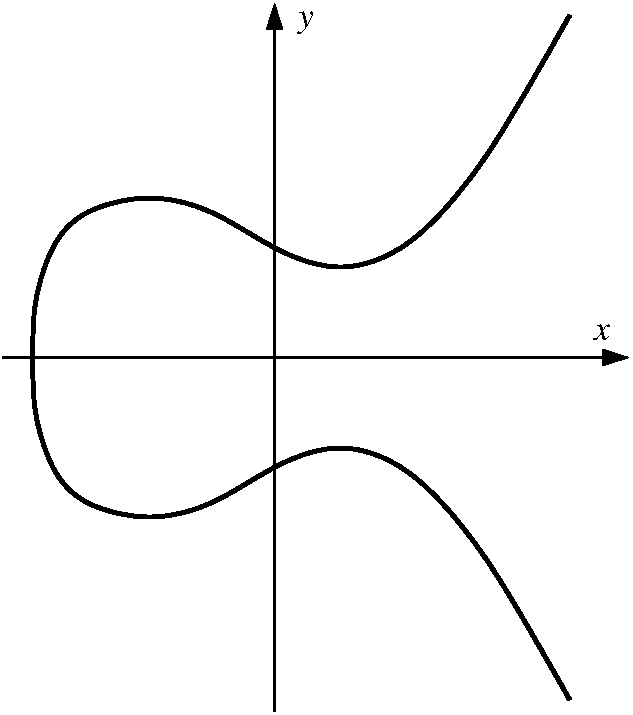
\includegraphics[scale=0.60]{figures/elliptic-curve}
\caption{Beispiel einer Elliptischen Kurve über dem Körper der reellen Zahlen}
\label{ExampleEllipticCurve}
\end{center}
\vskip -10 pt
\end{figure}
Als zugrunde liegenden Körper für eine Elliptische Kurve verwendet man in der Kryptographie stets endliche Körper $K=GF(p^n)$, also nicht wie in Abbildung \ref{ExampleEllipticCurve} die zu einer stetigen Kurve führenden reellen Zahlen. Der Grund liegt, einfach gesagt, darin, dass wir bei der Verarbeitung und Übertragung von Nachrichten stets nur endlich viele Zustände zur Verfügung haben (aufgrund der Arbeitsweise moderner Computer), Körper mit unendlich vielen Elementen wie z.B. die reellen Zahlen daher stets nur unvollständig darstellen können.

In der Praxis hat es sich als sinnvoll erwiesen, entweder $GF(p)$ mit einer großen Primzahl $p$ oder $GF(2^n)$ mit einer (großen) natürlichen Zahl $n$ zu betrachten. Der Grund für die Verwendung des Primkörpers $GF(p)$ liegt in seiner einfachen Arithmetik; andererseits kommt $GF(2^n)$ der binären Darstellung in Computersystemen entgegen. Andere Körper wie z.B. $GF(7^n)$ bieten keiner dieser beiden Vorteile und werden daher in der Praxis nicht verwendet, ohne dass dies theoretische Gründe hätte.

Durch Koordinatentransformation kann man die Weierstrass-Gleichung\index{Weierstrass, Karl} in einer einfacheren Form schreiben\footnote{Anschaulich bedeutet eine solche Koordinatentransformation eine Drehung bzw. Streckung der Koordinatenachsen, ohne dass die zugrunde liegende Kurve selbst verändert wird.}.  Je nachdem, ob $p>3$ ist, verwendet man unterschiedliche Transformationen und erhält so

\begin{itemize}
\item im Fall $GF(p)$, $p>3$, die Elliptische Kurven-Gleichung der Form
\begin{equation}
 y^2 = x^3 + ax + b
\label{ellp}
\end{equation}
mit $4a^3+27b^2\ne 0$
\item im Fall $GF(2^n)$ die Elliptische Kurven-Gleichung der Form
\begin{equation}
 y^2+xy = x^3 + ax^2 + b
\label{ell2}
\end{equation}
mit $b\ne 0$\footnote{Die Form (\ref{ellp}) ist die Standardform der Weierstrass-Gleichung\index{Weierstrass, Karl}. Ist die Charakteristik des Körpers jedoch $2$ oder $3$, so ist $4=0$ bzw. $27=0$, was dazu führt, dass man in der Bedingung an die Parameter $a,b$ wesentliche Informationen verliert. Dies ist ein Hinweis darauf, dass die Transformation auf die Standardform in diesen Fällen nicht zu befriedigenden Ergebnissen führt.}.
\end{itemize}
Durch diese Bedingungen an die Parameter $a,b$ ist gewährleistet, dass die Elliptische Gleichung für kryptographische Anwendungen geeignet ist\footnote{Formal sagt man, die Kurve ist nicht singulär.}.


Für die Anzahl $|E|$ der Elemente einer Elliptischen Kurve $E$ über einem Körper $GF(k)$ (praktisch $k=p$ prim oder $k=2^n$) gilt nach dem Satz von Hasse \cite{Silverman2009} die einfache Beziehung $| \, |E| - k-1\,| \le 2\cdot \sqrt{k}$. Diese Ungleichung ist äquivalent zu $k+1 - 2\sqrt{k} < |E| < k+1+2\sqrt{k}$. Dies bedeutet, dass die Anzahl der Elemente der Elliptischen Kurve mit der Größe $k$ gut abgeschätzt werden kann.

% $$ (\sqrt{k}-1)^2=k-2\sqrt{k}+1 \le |E| \le k+1 .
% $$
% Dies bedeutet, dass für große $k$ die Anzahl der Elemente der Elliptischen Kurve praktisch wie $k$ wächst.


% -----------------------------------------------------------------------------
\section{Verknüpfung auf Elliptischen Kurven}

Um mit Elliptischen Kurven arbeiten zu können, definiert man eine Verknüpfung (meist additiv als $+$ geschrieben) auf den Punkten der Elliptischen Kurve. Dabei definiert man bei Elliptischen Kurven über $GF(p)$ die kommutative Verknüpfung durch
\begin{enumerate}
\item $P+{\cal O}={\cal O}+P=P$ für alle $P\in E$,
\item für $P=(x,y)$ und $Q=(x,-y)$ ist $P+Q={\cal O}$,
\item für $P_1=(x_1,x_2),P_2=(x_2,y_2)\in E$ mit $P_1,P_2\ne {\cal O}$ und $(x_2,y_2)\ne (x_1,-y_1)$ ist $P_3:=P_1+P_2$, $P_3=(x_3,y_3)$ definiert durch
$$ x_3:=-x_1-x_2+\lambda^2 \, , \qquad y_3:=-y_1+\lambda (x_1-x_3)
$$
mit dem Hilfsquotienten
$$ \lambda:=\left\{ \begin{array}{cl} \frac{y_1-y_2}{x_1-x_2} & {\rm falls~} P_1\ne P_2,\\
                                     \frac{3x_1^2+a}{2y_1} & {\rm falls~} P_1=P_2. \end{array} \right.
$$
\end{enumerate}
Hieraus folgt insbesondere für $P=(x,y)\in E$, dass gilt $-P=(x,-y)$.

Über $GF(2^n)$ definiert man analog die Verknüpfung durch
\begin{enumerate}
\item $P+{\cal O}={\cal O}+P=P$ für alle $P\in E$,
\item für $P=(x,y)$ und $Q=(x,x+y)$ ist $P+Q={\cal O}$,
\item für $P_1=(x_1,x_2),P_2=(x_2,y_2)\in E$ mit $P_1,P_2\ne {\cal O}$ und $(x_2,y_2)\ne (x_1,x_1+y_1)$ ist $P_3:=P_1+P_2$, $P_3=(x_3,y_3)$ definiert durch
$$ x_3:=-x_1+x_2+\lambda+\lambda^2+a \, , \qquad y_3:=y_1+x_3+\lambda (x_1+x_3)
$$
mit
$$ \lambda:=\left\{ \begin{array}{cl} \frac{y_1+y_2}{x_1+x_2} & {\rm falls~} P_1\ne P_2,\\
                                   x_1+\frac{y_1}{x_1} & {\rm falls~} P_1=P_2. \end{array}\right.
$$
\end{enumerate}
Hieraus folgt insbesondere für $P=(x,y)\in E$, dass gilt $-P=(x,x+y)$.

(Beachte: $-(-P)=(x,x+(x+y))=(x,2x+y)=(x,y)$, da der zugrunde liegende Körper Charakteristik $2$ hat.)\footnote{%
Eine Animation der Punktaddition auf Elliptischen Kurven
findet man auf der Certicom-Seite\index{Certicom} unter\\
\url{https://www.certicom.com/ecc-tutorial} (Datum letzte Änderung unklar).\\
Vergleiche auch den Web-Link zum \hyperlink{ec:Web-Link:Java_Laubrock}
{Java-Tutorial} am Ende dieser Kapitels.

}

Man kann nachrechnen, dass die Menge $E\cap\{\cal O\}$ mit der so definierten
Addition eine Gruppe bildet. Dies bedeutet insbesondere, dass die Summe zweier
Kurvenpunkte stets wieder ein Punkt auf der Elliptische Kurve ist. Diese
Addition läßt sich auch geometrisch veranschaulichen, wie der folgende
Abschnitt zeigt.

% \newpage
\begin{figure}[htbp]
\subsection*{Addieren von Punkten auf einer Elliptischen Kurve}
Die zwei folgenden Abbildungen zeigen, wie bei einer Elliptischen Kurve über den reellen Zahlen in affinen Koordinaten
zwei Punkte addiert werden. Der unendlich ferne Punkt ${\cal O}$ kann nicht in der affinen
Ebene dargestellt werden.
\begin{center}
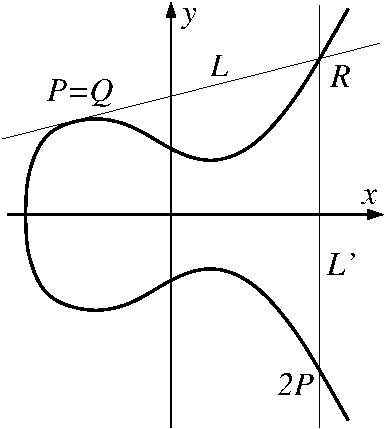
\includegraphics[scale=1.08]{figures/ec-mult2}
\caption{Verdoppelung eines Punktes}
\vspace{\floatsep}
\vskip +20 pt
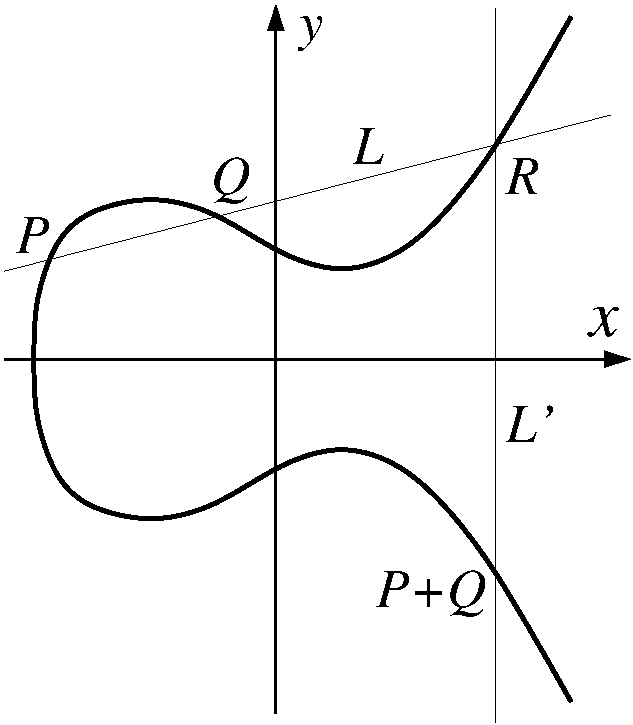
\includegraphics[scale=0.65]{figures/ec-add}  %be_2005 evtl. an diesem Vergrößerungsfaktor spielen
\caption{Addition zweier verschiedener Punkte im Körper der reellen Zahlen} % \footnotemark }
\end{center}
\end{figure}
% \addtocounter{footnote}{0}\footnotetext{Der Punkt $O$ kann nicht in der affinen Ebene dargestellt werden.}
\enlargethispage{+20pt}
\newpage


% -----------------------------------------------------------------------------
\section[Sicherheit der Elliptischen-Kurven-Kryptographie: Das ECDLP]{\sloppy Sicherheit der Elliptischen-Kurven-Kryptographie: Das ECDLP}

Wie bereits in Abschnitt \ref{ECC-Crypto} erwähnt, betrachten wir in der Kryptographie Elliptische Kurven über diskreten\footnote{Diskret im Gegensatz zu kontinuierlich.} Körpern $GF(2^n)$ oder $GF(p)$ (für große Primzahlen $p$). Dies bedeutet, dass alle Parameter, die zur Beschreibung der Elliptischen Kurve notwendig sind, aus diesem zugrunde liegenden Körper stammen. Ist nun $E$ eine Elliptische Kurve über einem solchen Körper und $P$ ein Punkt auf der Kurve $E$, so kann man für jede natürliche Zahl $m$
$$ mP := \underbrace{P+P+\dots+P}_{\hbox{$m$ mal}}
$$
bilden. Diese Operation ist aus kryptographischer Sicht deshalb besonders interessant, weil man einerseits um $mP$ zu berechnen im allgemeinen nur $\log m$ Additionen durchführen muss --- man bildet einfach $P$, $2P$, $2^2P$, $2^3P$, \dots, schreibt $m$ binär und addiert schließlich entsprechend der Binärdarstellung von $m$ auf --- es andererseits sehr aufwa"ndig zu sein scheint, zu gegebenen Punkten $P$ und $Q=mP$ auf $E$ die Zahl $m$ zu bestimmen. Natürlich kann man die Folge $P,2P,3P,4P,5P,\dots$ bilden und jeweils mit $Q$ vergleichen. Hierzu benötigt man jedoch $m$ Additionen.

Bisher ist noch kein Algorithmus bekannt, der effizient $m$ aus $P$ und $Q$ berechnet. Die bisher besten Verfahren liegen z.B. im Fall $GF(p)$ in der Größenordnung $\sqrt{q}$, wobei $q$ ein (großer) Primfaktor von $p-1$ ist; $m$ selbst sollte in diesem Fall zwischen $1$ und $q$ liegen, so dass man für die Muliplikation $mP$ maximal $\log q$ Schritte benötigt. Der Quotient $\frac{\sqrt{q}}{\log q}$ strebt jedoch (schnell) gegen $+\infty$.

Sind die Parameter hinreichend groß (ist zum Beispiel $p$ prim und
mehr als $160$ Bit lang) ist der Computer ohne weiteres in der Lage, sehr schnell (in wenigen
Bruchteilen einer Sekunden) den Punkt $mP$ zu bestimmen. Das {\it inverse Problem}, $m$ aus $mP$ und $P$ zu erhalten, ist jedoch nicht in akzeptabler Zeit möglich.

Dies wird als das \glqq Diskrete Logarithmus Problem über Elliptischen
Kurven\grqq\ bezeichnet (auch ECDLP\index{ECDLP} -- Elliptic Curve Discrete
Logarithm Problem -- abgekürzt).

\vskip +5 pt

Formal betrachten wir in der Elliptischen-Kurven-Kryptographie die Punkte der Kurve als Elemente einer Gruppe mit der Addition als Verknüpfung. Allerdings sind nur solche Elliptischen Kurven für kryptographische Anwendungen geeignet, bei der die Anzahl der Kurvenpunkte hinreichend groß ist. Ferner können in Spezialfällen Elliptische Kurven auch aus anderen Gründen ungeeignet sein. Das bedeutet, dass man bei der
Definition einer Kurve auf die Wahl der Parameter achten muss. Denn für bestimmte Klassen von
Elliptischen Kurven ist es möglich, das ECDLP leichter zu lösen als im allgemeinen Fall. Kryptographisch
ungeeignete Elliptische Kurven sind die sogenannten {\em anormalen} Kurven (das sind Kurven über ${\mathbb Z}_p$,
für die die Menge $\textbf{E}$ genau $p$ Elemente hat) und die {\em supersingulären} Kurven (das sind Kurven, für die man das
Berechnen des ECDLP auf das Berechnen des \glqq normalen\grqq\ Diskreten Logarithmus in anderen endlichen Körper
reduzieren, d.h. vereinfachen, kann). Daher gibt es kryptographisch gute und schlechte Kurven. Allerdings
kann man für gegebene Parameter $a$ und $b$ mit etwas Aufwand feststellen, ob die resultierende Elliptische
Kurve kryptographisch brauchbar ist oder nicht. Die in der Kryptographie eingesetzten Kurven werden meist
von Fachleuten zur Verfügung gestellt. Sie gewährleisten, dass die von ihnen als sicher eingestuften
Elliptischen Kurven den aktuellen Sicherheitsanforderungen genügen.
\vskip +5 pt

Bei sicheren Kurven wird hauptsächlich
durch den Parameter $p$ im Fall des zugrunde liegenden Körpers $GF(p)$ bzw. $n$ im Fall des zugrunde liegenden Körpers $GF(2^n)$ bestimmt, wie lange es dauert, das ECDLP auf dieser Kurve zu lösen. Je größer diese
Parameter sind, desto länger nimmt das Lösen des Problems in Anspruch. Von Fachleuten wird z.B. eine Bitlänge
von über $200$ Bit für den Parameter $p$ empfohlen. Hier wird deutlich, warum die Elliptischen Kurven so
interessant für die Kryptographie sind. Denn die Parameter bestimmen auch den
Signatur-/Verschlüsselungsaufwand, wenn mit Elliptischen Kurven
Kryptographie betrieben wird. Die Dauer einer Schlüsselpaar-Erzeugung ist ebenfalls von den Parametern abhängig. Daher sind kleine Werte (wenige Bits) wünschenswert (möglichst schnelle Laufzeiten der Verfahren);
allerdings muss die geforderte Sicherheit dabei eingehalten werden.
Mit einer Länge von zum Beispiel $200$ Bit für $p$ ist eine {\em gute} Elliptische Kurve
genau so sicher wie ein \index{RSA!Modulus} RSA-Modulus von über $1024$ Bit Länge
(zumindest nach dem heutigen Forschungstand). Der Grund dafür ist, dass die schnellsten
Algorithmen zum Lösen des {\em Elliptische Kurven Diskreter Logarithmus}-Problems eine
exponentielle Laufzeit haben --- im Gegensatz zu den subexponentiellen Laufzeiten, die
die zur Zeit besten Faktorisierungsalgorithmen haben (Zahlkörpersieb, Quadratisches Sieb
oder Faktorisieren mit Elliptischen Kurven). Dies erklärt, warum die Parameter von
Kryptoverfahren, die auf dem Problem {\em Faktorisieren von ganzen Zahlen} beruhen,
größer sind als die Parameter von Kryptoverfahren, die auf dem ECDL-Problem basieren.


% -----------------------------------------------------------------------------
\section{Verschlüsseln und Signieren mit Hilfe Elliptischer Kurven}

\begin{sloppypar}
  Das {\em Elliptische Kurven Diskreter Logarithmus
    Problem}\index{Logarithmusproblem} (ECDLP) \index{ECDLP} ist die
  Grundlage für die Elliptische-Kurven-Kryptographie. Darauf basierend gibt es verschiedene Signaturverfahren. Um ein solches Signaturverfahren anzuwenden, benötigt man:
\end{sloppypar}
\begin{itemize}
    \item Eine Elliptische Kurve \textbf{E}, beschrieben durch den zugrunde liegenden Körper $GF(p^n)$.
    \item Eine Primzahl $q\ne p$ sowie einen Punkt $G$ auf der Elliptischen Kurve $\textbf{E}$ mit Ordnung $q$. D.h., es gilt $qG={\cal O}$ und $rG\ne {\cal O}$ für alle $r\in \{1,2,\dots,q-1\}$. Die Zahl $q$ muss dann ein Teiler der Gruppenordnung (entspricht der Anzahl der Elemente) $\#\textbf{E}$ sein. Aufgrund der Primordnung, erzeugt $G$ eine zyklischen Untergruppe von $\textbf{E}$ mit Ordnung $q$.
\end{itemize}
Die genannten Parameter bezeichnet man als \index{Domain-Parameter} {\em Domain}-Para\-meter. Durch sie wird
festgelegt, auf welcher Elliptischen Kurve $\textbf{E}$ und in welcher zyklischen Untergruppe von $\textbf{E}$ ein
Signaturverfahren eingesetzt  wurde.

\par
%\smallskip
%\textbf{Verschlüsselung:}
\subsection{Verschlüsselung}

Mit Hilfe Elliptischer Kurven kann ein sicherer Schlüsselaustausch nach dem \hyperlink{DH-KeyExch}{Diffie-Hellman}-Protokoll \index{Diffie-Hellman} erfolgen (siehe Kapitel \ref{DH-KeyExch}). Dieser Schlüssel kann dann für eine anschließende symmetrische Verschlüsselung verwendet werden. Ein Schlüsselpaar mit privatem und öffentlichem Schlüssel wird im Gegensatz zum RSA-Algorithmus nicht erzeugt!

In der Schreibweise der Elliptischen Kurven liest sich das Diffie-Hellman Verfahren wie folgt: Zunächst einigen sich beide Partner (A und B) öffentlich auf eine Gruppe $G$ und eine ganze Zahl $q$. Danach wählen sie zufällig $r_A,r_B\in\{1,2,\dots,q-1\}$, bilden die Punkte $R_A=r_AG$, $R_B=r_BG$ auf der Elliptischen Kurve und tauschen diese aus. Danach berechnet A leicht $R=r_AR_B$. Denselben Punkt (nämlich $r_Ar_B G$) erhält auch B, indem er $r_BR_A=r_Br_AG=r_Ar_BG=R$ bildet. Dabei ist die Berechnung von $R_A,R_B$ als $r_A$ bzw. $r_B$-faches des Kurvenpunktes $G$ leicht durchzuführen; die umgekehrte Operation, aus $R_A$ bzw. $R_B$ den Wert $r_A$ bzw. $r_B$ zu erhalten, ist jedoch sehr aufwändig.
\\ Für einen Dritten ist es nach heutigen Kenntnisstand nicht möglich, $R$ zu berechnen, wenn er nicht mindestens einen der Werte $r_A$ oder $r_B$ ermitteln kann, d.h. das ECDLP löst.

Um einen \glqq Man-in-the-Middle\grqq-Angriff zu verhindern, kann man auch hier wie schon in Kapitel \ref{Impersonalisierungsattacke} beschrieben, die übertragenen Werte $G,q,R_A,R_B$ digital signieren.

\par
%\smallskip
%\textbf{Signatur-Erstellung:}
\subsection{Signatur-Erstellung}

Überträgt man den \index{DSA} DSA auf Elliptische Kurve, so kann man wie folgt eine digitale Signatur erzeugen: Man wählt vorab eine (nicht-triviale) Zahl $s\in{\mathbb Z}_q$. Diese bildet den privaten Schlüssel. Hingegen werden $q$, $G$ und $R=sG$ veröffentlicht. Aus $G$ und $R$ lässt sich jedoch $s$ nicht ermitteln, worauf die Sicherheit des Signaturverfahrens beruht.

Für eine Nachricht $m$ wird zunächst mit Hilfe eines Hash-Verfahrens $h$ ein digitaler Fingerabdruck erstellt, wobei $h(m)$ im Wertebereich $\{0,1,2,\dots, q-1\}$ liegt und $h(m)$ somit als Element von ${\mathbb Z}_q$ interpretiert werden kann. Dann wird ein zufälliges $r\in{\mathbb Z}_q$ gewählt und $R=(r_1,r_2)=rG$ berechnet. Die erste Komponente $r_1$ von $R$ ist ein Element von $GF(p^n)$. Diese wird auf ${\mathbb Z}_q$ abgebildet, z.B. im Fall $n=1$ als Element von $\{0,1,\dots,p-1\}$ interpretiert und dann der Teilerrest modulo $q$ gebildet. Das so erhaltene Element von ${\mathbb Z}_q$ bezeichnen wir mit $\bar r_1$. Nun bestimmt man $x\in {\mathbb Z}_q$ mit
$$ rx-s\bar r_1-h(m)=0 .
$$
Das Tripel $(m,r_1,x)$ bildet nun die digitale Signatur.

\par
%\smallskip
%\textbf{Signatur-Verifikation:}
\subsection{Signatur-Verifikation}

Zur Verifikation muss zunächst $u_1=h(m)/x$, $u_2=\bar r_1/x$ (in ${\mathbb Z}_q$ gebildet werden). Dann bestimmt man
$$ V=u_1G+u_2Q .
$$
Wegen $Q=sG$ ist $V=(v_1,v_2)$ mit $v_1=u_1+u_2s$. Diese Addition findet formal im Raum $GF(p^n)$ statt. Die Projektion von $GF(p^n)$ auf ${\mathbb Z}_q$ sollte jedoch so gewählt sein, dass $\bar v_1=u_1+u_2s$ in ${\mathbb Z}_q$ ist.
Dann gilt nämlich
$$ \bar v_1=u_1+u_2s=h(m)/x+\bar r_1 s/x=(h(m)+\bar r_1s)/x=rx/x=r .
$$
Nun ist $R=rG$. Also folgt hier $\bar v_1=\bar r_1$, d.h. $R$ und $V$ stimmen modulo der Projektion auf ${\mathbb Z}_q$ überein.


% -----------------------------------------------------------------------------
\hypertarget{faktell}{}
\section{Faktorisieren mit Elliptischen Kurven} \label{ECC-Factorisation}

Es gibt Faktorisierungsalgorithmen%
\footnote{John M. Pollard \index{Pollard, John M.} war an der
Entwicklung vieler verschiedener Faktorisierungsalgorithmen beteiligt; auch
beim Faktorisieren mit ECC war er einer der führenden Köpfe. Als Mitarbeiter
von British Telekom hat er leider nie viel selbst publiziert. Auf der RSA
Konferenz 1999 wurde er für seine \glqq outstanding contributions in
mathematics\grqq~ausgezeichnet.\\
Im Jahr 1987 stellte H.W. Lenstra\index{Lenstra 1987} einen häufig genutzten
Faktorisierungsalgorithmus vor, der auf Elliptischen Kurven basiert
(siehe \cite{Lenstra1987}).
  % Leerzeile vor schließender Footnote-Klammer zu #21 nötig, um einheitlich eine
  % Leerzeile am Ende der Fußnoten zu haben -- solange keine andere Lösung
  % für das Einrückproblem bei Fußnote #23 (TODO_LaTeX)

}, die auf Elliptischen Kurven
\index{Faktorisierung!Faktorisierungsalgorithmen} basieren\footnote{%
Die größten mit Elliptischen Kurven faktorisierten
Zahlen\index{Faktorisierung!Faktorisierungsrekorde} haben ca. 80 Dezimalstellen:\\
\url{https://members.loria.fr/PZimmermann/records/top50.html}.\\
% \url{http://www.loria.fr/~zimmerma/records/top50.html}.\\
Vergleiche auch den Web-Link über das \hyperlink{Lenstra2}{ECMNET-Projekt}
\index{ECMNET} am Ende dieser Kapitels.
}.
Genauer gesagt, machen sich diese Verfahren zunutze, dass man auch
über ${\mathbb Z}_n$ ($n$ zusammengesetzte Zahl) Elliptische Kurven
definieren kann. Elliptische Kurven über ${\mathbb Z}_n$ bilden keine
Gruppe, da es nicht zu jedem Punkt auf solchen Elliptischen Kurven einen
inversen Punkt geben muss. Dies hängt damit zusammen, dass es -- falls $n$
eine zusammengesetzte Zahl ist -- in ${\mathbb Z}_n$ Elemente gibt, die
kein Inverses bezüglich der Multiplikation modulo $n$ haben. Um zwei
Punkte auf einer Elliptischen Kurve über ${\mathbb Z}_n$ zu addieren, kann
prinzipiell genauso gerechnet werden wie auf Elliptischen Kurven über
${\mathbb Z}_p$. Eine Addition von zwei Punkten (auf einer Elliptischen
Kurve über ${\mathbb Z}_n$) scheitert aber genau dann, wenn man einen
Teiler von $n$ gefunden hat. Der Grund dafür ist, dass das Verfahren zum
Addieren von Punkten auf Elliptischen Kurven Elemente in ${\mathbb Z}_n$
ermittelt und zu diesen Elementen die inversen Elemente (bezüglich der
Multiplikation modulo $n$) in ${\mathbb Z}_n$ berechnet. Dazu wird der
erweiterte \index{Euklidscher Algorithmus} Euklidsche Algorithmus benutzt.
Ergibt sich nun bei der Addition zweier Punkte (die auf einer Elliptischen
Kurve über ${\mathbb Z}_n$ liegen) ein Element aus ${\mathbb Z}_n$, das
kein inverses Element in ${\mathbb Z}_n$ hat, so gibt der erweiterte
Euklidsche Algorithmus\index{Euklidscher Algorithmus!erweiterter}
einen echten Teiler von $n$ aus.

Das Faktorisieren mit Elliptischen Kurven funktioniert somit prinzipiell so: Man wählt zufällige Kurven
über ${\mathbb Z}_n$, sowie zufällig irgendwelche Punkte (die auf diesen Kurve liegen) und addiert diese; dabei
bekommt man wieder Punkte, die auf der Kurve liegen oder findet einen Teiler von $n$. Die
Faktorisierungsalgorithmen auf Basis von Elliptischen Kurven arbeiten also probabilistisch.
Durch die Möglichkeit, sehr viele Elliptische Kurven über ${\mathbb Z}_n$ zu definieren, kann man die
Wahrscheinlichkeit erhöhen, zwei Punkte zu finden, bei deren Addition ein Teiler von $n$ gefunden wird.
Daher eignen sich diese Verfahren auch sehr gut für eine Parallelisierung.


% -----------------------------------------------------------------------------
\newpage
\section{Implementierung Elliptischer Kurven zu Lehrzwecken}
\label{ec:Implementing-for-Education}

Es gibt relativ wenig freie Programme mit graphischer Oberfläche, die ECC implementieren.
Im Folgenden wird aufgezeigt, welche Funktionalität
dazu in CrypTool und in SageMath vorhanden ist.


% -----------------------------------------------------------------------------
\subsection{CrypTool}\index{CrypTool}

CT1 enthält Elliptische Kurven, um digitale Signaturen zu erzeugen%
\footnote{%
Die Dialogbox, die in CT1\index{CT1} nach dem Menü
\textbf{Digitale Signaturen/PKI \textbackslash{} Dokument signieren} erscheint,
bietet die EC-Verfahren ECSP-DSA und ECSP-NR an.
} und um die ECC-AES-Hybridverschlüsselung durchzuführen%
\footnote{%
In CT1\index{CT1} finden Sie dieses Verfahren über das Menü
\textbf{Ver-/Entschlüsseln \textbackslash{} Hybrid}.
}.

Implementiert sind die Basisalgorithmen für Gruppenoperationen, für das
Erzeugen von Elliptischen Kurven und für das Ein- und Auslesen von
Parametern für Elliptische Kurven über endlichen Körpern $GF(p)$
mit $p$ Elementen ($p$ prim). Die Implementierung erfolgte in
ANSI C und richtete sich nach dem Entwurf Nr. 8 der Arbeitsgruppe
IEEE P1363 {\em Standard Specifications for Public Key Cryptography}.
%% BE: Link raus, da tot: {\url{http://grouper.ieee.org/groups/1363}}.

Implementiert sind die kryptographischen Primitive zur Signaturerzeugung
und Signaturverifikation für die auf Elliptischen Kurven basierenden
Varianten von Nyberg-Rueppel-Signaturen und \index{DSA} DSA-Signaturen.

Schritt-für-Schritt ist die Punkt-Addition auf elliptischen Kurven
in CT1\index{CT1} and JCT\index{JCT} visualisiert.%
\footnote{%
  CT1: Menü \textbf{Digitale Signaturen/PKI \textbackslash{} Signaturdemo
  (Signaturerzeugung)},\\
  JCT (Standard-Perspektive): Menü \textbf{Visualisierungen \textbackslash{}
  Elliptische Kurven-Berechnungen}.
}


% -----------------------------------------------------------------------------
\subsection{SageMath}
\label{ec:Sage_Massierer}
\index{SageMath}
\index{SageMath!Programmbeispiele}

In SageMath finden sich sehr gute Beschreibungen über Elliptische Kurven unter:%
\footnote{%
SageMath-Beispiele dazu finden sich z.B. auch in
  dem \glqq Elliptic Curve Cryptography (ECC) Tutorial\grqq\\
  \url{http://www.williamstein.org/simuw06/notes/notes/node12.html}
}

\begin{sloppypar} % Nötig, da der 2. Link sonst nicht umgebrochen.
\begin{itemize}
    \item \url{http://doc.sagemath.org/html/en/constructions/elliptic_curves.html}
    \item \url{http://doc.sagemath.org/html/en/reference/curves/index.html#elliptic-curves}
\end{itemize}
\end{sloppypar}


Zusätzlich gibt es ein ausführliches, interaktives
\hyperlink{ec:Web-Link:Sage_Massierer}{ECC-Tutorial} von Maike Massierer.
Diese Einführung in die Elliptische-Kurven-Kryptographie (ECC)
ist als SageMath-Notebook aufgebaut.

SageMath-Notebooks werden im Browser nach einem Logon-Vorgang aufgerufen%
\footnote{%
Hat man SageMath auf einem eigenen (Unix-)Server installiert, muss
man auf der SageMath-Kommandozeile erst den Befehl \verb#notebook()# aufrufen.
}${}^,$\footnote{%
Das \hyperlink{ec:Web-Link:Sage_Massierer}{ECC-Notebook} von Massierer
benötigt die KASH3-Bibliothek: Deshalb muss (z.B. für SageMath 4.2.1)%TODO-Version
das Package \glqq kash3-2008-07-31.spkg\grqq~installiert
worden sein (Befehl \verb#sage -i#).
}.


%--------------
Das \hyperlink{ec:Web-Link:Sage_Massierer}{ECC-Notebook}
\index{elliptische Kurve!ECC-Notebook}\index{Massierer, Maike}
wurde 2008 von Massierer\footnote{%
Anleitung zur Benutzung eines interaktiven SageMath-Notebooks\index{SageMath!Anleitung interaktives Notebook}:
Aktualisieren für die neue SageMathCloud xxxxxxxxxxxxx\\
%todoTODO
\begin{itemize}
  \item[-] Manche SageMath-Server sind öffentlich
  und bieten Worksheets als
  \glqq Published Worksheets\grqq~ an, die man ohne Log-in
  ausführen kann. Diese Worksheets werden aufgelistet, wenn man
  auf \glqq Published\grqq~in der oberen rechten Ecke klickt.
  \item[-] Worksheets, die den  \verb#Interact#-Befehl nutzen, erfordern z.Zt.
  einige weitere Schritte vom Benutzer: Einloggen, Kopie erstellen,
  alle Kommandos nochmal ausführen.\\
\item[-]
  Teile des ECC-Tutorial benutzen einen speziellen Mathematik-Font, der standardmäßig
  bei den meisten Browser nicht mitinstalliert wird. Wenn Sie bemerken, dass Formeln
  nicht korrekt dargestellt sind oder Ihr Browser meldet, dass Fonts fehlen,
  installieren Sie bitte die Fonts jsMath für eine bessere Darstellung.\\
  Siehe \url{http://www.math.union.edu/~dpvc/jsMath/}.\\
  Nach der Installation dieser Fonts hat man das jsMath-Symbol am unteren Rand
  des Browsers. Klickt man dieses Symbol an, erhält man die Download-Seite dieser
  TIFF-Fonts. Diese Font-Installation muss an jedem PC einzeln erfolgen.
\end{itemize}
}
erstellt und besteht aus 8 Teilen (\glqq Titelseite\grqq~mit Inhaltsverzeichnis
plus 7 Kapitel) und zielt darauf ab, dass selbst ein Einsteiger versteht, was
Elliptische Kurven sind (es ist nur auf Englisch vorhanden):
\begin{enumerate}
   \setcounter{enumi}{-1}
   \item ECC Notebook (title page and contents)
   \item Introduction and Overview
   \item Motivation for the use of Elliptic Curves in Cryptography
   \item Elliptic Curves in Cryptography
   \item Cryptographic Protocols in ECC
   \item Domain Parameter Generation for ECC Systems
   \item Conclusion and Further Topics
   \item References
\end{enumerate}


% -----------------------------------------------------------------------------
\newpage
\section{Patentaspekte}\index{Patent}

Wenn man statt des Primkörpers $GF(p)$ einen Körper der Form $GF(2^n)$ zugrunde legt, ergeben sich wesentliche Unterschiede in der Implementierung. Der Vorteil einer Implementierung unter Verwendung von $GF(2^n)$ liegt darin, dass Rechnungen aufgrund der binären Darstellung effizienter durchgeführt werden können. Dies betrifft insbesondere die Division, die in $GF(p)$ vergleichsweise aufwändig ist (was z.B. bei dem oben beschriebenen Signaturverfahren sowohl die Erstellung der Signatur als auch ihre spätere Verifikation betrifft, da beide eine Divisionsoperation enthalten).

Um das Potenzial der Effizienzsteigerung möglichst optimal zu nutzen, kann man z.B. Körper wählen, die besondere Basen besitzen, wie Polynomialbasen (besonders geeignet für Software-Implementierungen) oder Normalbasen (bevorzugt bei Hardware-Implementierungen). Für bestimmte Werte von $n$ (wie z.B. $n=163,179,181$) lassen sich sogar beide Vorteile kombinieren. Allerdings sind spezielle Darstellungen oft nicht Standard.

Um Speicherplatz zu sparen, wird zuweilen nur die erste Komponente sowie ein weiteres Bit für jeden Punkt auf der Elliptischen Kurve gespeichert. Hieraus kann jeweils der gesamte Punkt errechnet werden. Dies ist besonders bei Verwendung von Normalbasen effizient. Selbst bei der Durchführung der kryptographischen Protokolle kann eine signifikante Beschleunigung erreicht werden. Diese sogenannte {\it Punkt-Kompression}, die bei der Hälfte aller Kurven einsetzbar ist, ist jedoch patentiert (US Patent 6141420, Certicon) und daher nicht ohne weiteres frei einsetzbar.

Im allgemeinen Fall $GF(p^n)$ (aber auch für $n=1$) werden oft sogenannte affine oder projektive Koordinaten eingesetzt, was je nach Anwendung zu Effizienzgewinnen führt.

Eine vollständige Beschreibung aller Implementierungen unter Abwägung ihrer Vor- und Nachteile würde an dieser Stelle zu weit führen. Abschließend kann festgehalten werden, dass die Vielfalt möglicher Implementierungen bei Elliptischen Kurven z.B. im Vergleich zu RSA-Implementie"-rungen sehr groß ist. Aus diesem Grund gibt es Bestrebungen, sich auf wenige Standardimplementierungen, ja sogar auf eine kleine Schar fest vorgegebener Kurven zu beschränken (ASC-Ansatz).

Der Erfolg dieser Standardisierungsbemühungen ist noch nicht absehbar.
Dies wäre aber eine Voraussetzung dafür, dass sich ECC dauerhaft als
Alternative zu RSA etabliert. Die Arbeit der Standardisierungskomitees wird
sich erheblich beschleunigen müssen, wenn sich abzeichnet, dass die aktuellen
Forschungsprojekte im Bereich der Faktorisierung einen Durchbruch erzielen.

Aktuelle Informationen zur Patentlage finden sich hier\footnote{%
\url{https://en.wikipedia.org/wiki/Elliptic_curve_cryptography}\\
\url{https://en.wikipedia.org/wiki/ECC_patents}\\
\url{https://cr.yp.to/ecdh/patents.html} Bernstein, Daniel J. (2006-05-23):
\glqq Irrelevant patents on elliptic-curve cryptography\grqq. Abgerufen 2016-07-14.
}.


% -----------------------------------------------------------------------------
\section{Elliptische Kurven im praktischen Einsatz}

% Einsatz in Protokollen wie TLS, Chats, ... ergänzen !!  xxxxxxxxxxxxxxxxxxxxxxxxx
Bereits heute werden Elliptische Kurven in der Praxis breit eingesetzt.
Als prominentes Beispiel ist hier der Informationsverbund Bonn-Berlin (IVBB)\footnote{%
Der IVBB verbindet Regierungsstellen in der alten und neuen deutschen Hauptstadt.\\
% Link tot: \url{http://www.cio.bund.de/cln_094/sid_92C19118CBA5A021AFD1ABAEC15D2B77/DE/IT-Angebot/IT-Infrastrukturen/IVBB/ivbb_inhalt.html}
}\index{IVBB} zu nennen, bei dem
streng vertrauliche Dokumente der deutschen Bundesregierung zwischen Regierungsstellen
mit Sitz in Berlin und Bonn ausgetauscht werden. Durch den Einsatz von ECC konnte eine
Hochsicherheitslösung realisiert werden. Fragen der Interoperabilität spielten
hingegen eine untergeordnete Rolle.

In Österreich gibt es eine Massenanwendung auf Basis von ECC: Die Bankkarte mit Signaturfunktion.

Beide Beispiele zeigen typische Einsatzgebiete Elliptischer Kurven:
Als Hochsicherheitslösungen und bei Implementierungen auf Smartcards, bei denen
der Schlüssellänge (begrenzter Speicherplatz) eine entscheidende Bedeutung zukommt.



%------------------------------------------------------------------------------
\printbibliography[%
	heading=subbibintoc,
	title={Literatur zu Kapitel \thechapter},
	segment=\therefsegment,
]


Alle Links wurden am 14.07.2016 überprüft.



%--------------------------------------------------------------------
\chapter*{Web-Links}
\addcontentsline{toc}{section}{Web-Links}

\begin{enumerate}

   \hypertarget{ec:Web-Link:Sage_Massierer} %% to be referred via \hyperlink
   %  -> Zum Ansehen: (siehe Massierers Mail vom 05.09.2008 12:52).
   \item Umfassende interaktive Einführung in elliptische Kurven und
        Elliptische-Kurven-Krypto"-graphie (ECC) mit SageMath\index{SageMath}
        von Maike Massierer und dem CrypTool-Team (alles in Englisch).\\
        ECC-Tutorial als SageMath-Notebook, Version 1.3, Januar 2011
        \url{http://web.maths.unsw.edu.au/~maikemassierer/ecc-notebook/}\\

   \hypertarget{ec:Web-Link:Certicom_Tutorial}{}
   \item Online-Tutorial über Elliptische Kurven der Firma
        Certicom\index{Certicom} (alles in Englisch),\\
	\url{https://www.certicom.com/index.php/ecc-tutorial}

   \hypertarget{ec:Web-Link:RSALabs}{}
   \item Overview of Elliptic Curve Cryptosystems,\\
        Revised June 27, 1997.~
        M.J.B. Robshaw und Yiqun Lisa Yin.\\
        RSA Laboratories\index{RSA Laboratories} (alles in Englisch),
        \begin{sloppypar} % To avoid black boxes because of long urls. If used, take away // before.
        \url{http://www.emc.com/emc-plus/rsa-labs/historical/overview-elliptic-curve-cryptosystems.htm}
        \end{sloppypar}

   \hypertarget{ec:Web-Link:Java_Laubrock}{}
   \item Tutorial mit Java Applets -- Krypto-Verfahren basierend auf
        elliptischen Kurven,\\
        Diplomarbeit Thomas Laubrock, 1999,\\
        \url{http://www.warendorf-freckenhorst.de/elliptische-kurven/frame.html}

   \item Arbeitsgruppe IEEE P1363,\\
        IEEE P1363 ist ein IEEE Standardisierungs-Projekt für Public-Key-Kryptographie.\\
		Elliptische Kurven waren Teil von sogenannten established oder traditional Public-Key-Dokumenten. Das Projekt begann 1993. Die ursprüngliche Webseite der Gruppe \nolinkurl{http://grouper.ieee.org/groups/1363} ist nicht mehr erreichbar (Stand 2018-08-08).

   \item \hypertarget{Lenstra2} Eine informative Seite zum Faktorisieren mit
        Elliptischen Kurven,\\
        Dort findet man Literatur zum Thema Faktorisieren mit Elliptischen
	Kurven sowie Links zu anderen ECC-Seiten.\\
        \url{https://members.loria.fr/PZimmermann/records/ecmnet.html}

   \item BSI TR-02102-1,\\
	Technische Richtlinie \glqq Kryptographische Verfahren: Empfehlungen
        und Schlüssellängen\grqq\\
	15. Februar 2016.\index{BSI}
        % BSI -- Technische Richtlinie
        % Bezeichnung:  Kryptographische Verfahren: Empfehlungen und Schlüssellängen
        % Kürzel:       BSI TR-02102-1
        % Version:      2016-01
        % Stand:        15. Februar 2016
        \begin{sloppypar} % To avoid black boxes because of long urls. If used, take away // before.
        \url{https://www.bsi.bund.de/DE/Publikationen/TechnischeRichtlinien/tr02102/index_htm.html}\\
        \url{https://www.bsi.bund.de/SharedDocs/Downloads/DE/BSI/Publikationen/TechnischeRichtlinien/TR02102/BSI-TR-02102.pdf?__blob=publicationFile&v=2}
        \end{sloppypar}

\end{enumerate}

Alle Links wurden am 06.08.2018 überprüft.

\end{refsegment}
% Local Variables:
% TeX-master: "../script-de.tex"
% End:
